%\chapterauthor{Author Name}{Author Affiliation}
%\chapterauthor{Second Author}{Second Author Affiliation}
\chapter{Trend Identification}

Statistically it has been a classic problem to distinguish \textit{trends} from \textit{variances} when one looks at the historical prices of any financial instrument. The price trajectory is hence usually regarded as non-stationary and treated in a stochastic way. For instance, in the classical Black-Scholes world a stock price is usually modelled as a Geometric Brownian Motion, with log-normal variations around an exponential trend. However, intuitively it seems also quite obvious that certain trends do exist, which are naturally important for investment decisions.

In this chapter we discuss a straightforward approach to automatically identify the trends in a price trajectory based on the identification of local minimums / maximums. We then investigate the empirical facts of such trends for stock indices as well as famous individual stocks. In subsequent chapters, we will build up a model based on logistic regression and other machine learning techniques to identify the potential trend using financial and economic variables as risk drivers. 

It should be noted that trend identification has been investigated in the technical analysis. Conventional methods include making use of moving averages, momentum indicators, trendlines and chart patterns via visual inspection (e.g. "higher highs and higher lows"). The difference however is that those techincal analysis methods usually aim to help identify short-term market anomalies e.g. overbought or oversold signals, while in this chapter the purpose is to structurally quantify the upward / downward trends and furthermore link them with potential risk drivers. 

\section{Reflection Points and Trends}\label{Definitions}

Motivated by the idea that any unilateral trend would start with a low/high point and end at a high/low point, we start with defining local minimums/maximums. 

Consider a price trajectory $\{S_t\}$ is observed. We have the following definition: 

\begin{definition}
	\label{RP}
	\textbf{(Reflection point.)} A price $S_t$ is called a \textbf{minimum/maximum reflection point of period $\tau$} (MIRP / MARP in short) if it is the minimum/maximum of the price in the period $[t-\tau, t+\tau]$. 
\end{definition}

By definition such reflection points are local extremes within a certain time window. It's also clear that they are subject to the choice of time window: a reflection point of a longer time window is also one for a shorter time window, but not vice versa. 

It's tempting to already identify a \textit{trend} by dividing the entire trajectory into pieces according to adjacent MARPs or MIRPs. However, such definition of reflection points focuses only on the local behaviour of the price trajectory and it's far from sufficient to always be able to use them for meaningful trend identification. In particular, there is no guarantee that 
\begin{itemize}
	\item the local minimums and maximums are always distributed in a "crossed" way, i.e. it can happen that two local minimums lie adjacent with no local maximum in between (\textit{duplicated RPs}). An example is a W-shaped price curve, with a relatively low high between two local minimums.
	\item a local minimum / maximum is always lower / higher than its adjacent local maximum / minimum (\textit{irregular RPs}). Exceptional cases are rare, but can happen when a relatively short horizon is chosen. 
\end{itemize}

Ideally, we would like to find \textit{meaningful} reflection points that helps to identify trends in a reasonable way. This leads to the following definition. 

\begin{definition}
	\label{vRP}
	\textbf{(Validated reflection point.)} A reflection point is called a \textbf{validated maximum / minimum reflection point} (vMARP / vMIRP in short) if it has a lower minimum / higher maximum reflection point as its preceding and subsequent reflection points. 
\end{definition}

We can then define a trend based on the validated reflection points. Note that the definition of the validated reflection point guarantees that the entire price trajectory can be divided into either upward or downward trends -- except the piece before the first and after the last reflection point. 

\begin{definition}
	%\label{RP}
	\textbf{(Trend.)} A piece of price trajectory is called a(n) \textbf{upward / downward trend} if it starts with a vMIRP / vMARP (inclusive) and ends with a vMARP / vMIRP (exclusive). 
\end{definition}

To get the validated RPs, the identified RPs needs to be filtered. For the first issue mentioned above (i.e. duplicate RPs), there are two ways to deal with this: 
\begin{itemize}
	\item keep the lowest MIRP / highest MARP and drop all the others in case of adjacent same local extremes; 
	\item identify the piece of price trajectory between two MARPs/MIRPs as a separate \textit{flat trend} next to the upward and downward ones.  
\end{itemize}

The drawback of the second treatment is that it will create a 3-state value space for the trends instead of a 2-state space consisting of only upwards and downwards. To optimally use the available historical data we choose to go with the first treatment, i.e. only keep the lowest MIRP / highest MARP. 

It is also a possibility to keep all the identified RPs and identify a new maximum / minimum between two adjacent MIRPs / MARPs. The drawback is however that it will then lead to ``false" RPs (i.e. which do not qualify to be a reflection point) and thus leads to ``false" trends. Hence we choose to drop the redundant local RPs and keep only the meaningful ones. 

The second issue (i.e. irregular RPs) usually happens when there are short-period turbulences in a long-period trend. For instance, a MARP is identified at an early stage of a long upward trend, and a MIRP is subsequently identified at a later stage, simply due to temporarily increasing market volatility. The strong upward trend however prevents to identify a \textit{lower} MIRP after that MARP, and the same holds for the MIRP at the later stage. The result is that a wrong downward trend can be identified -- which begins with a local maximum and ends with a local minimum -- while it's actually an upward trend. 

To deal with this issue we choose to drop both the reflection points in case a MARP is lower than an subsequent MIRP or a MIRP is higher than an subsequent MARP. The rationale is that, though those reflection points are local extremes, in most cases they cannot be used to identify meaningful trends in the price trajectory. 

We then have an algorithm to filter the RPs to get the validated ones: 
\begin{enumerate}
	\item Divide the RPs into groups based on whether they are adjacent local MARPs / MIRPs. If there are multiple MARPs / MIRPs in any group, keep the highest / lowest one and drop all the others. 
	\item For the remaining RPs, drop the ''irregular" ones, i.e. if a MARP is lower than its subsequent MIRP, or a MIRP is higher than its subsequent MARP. 
\end{enumerate}

It is not the purpose to provide a rigorous mathematical proof to show that such way to find the validated RPs is in any sense optimal. Nonetheless, it can be shown that such a way is sufficient to filter out validated RPs, based on which we can identify meaningful trends. 

The trends defined in this section should however be interpreted carefully. Any trend would start with a vMIRP and end with a vMARP (or vice versa), which are all the local extremes if one looks at a period of $\tau$ before and after that time. This means that this identified trend cannot be further extended forwards or backwards in time at least within a period of $\tau$. The duration of the trend, on the other hand, can be of any duration, even shorter than $\tau$. 

A larger $\tau$ would indicate a stronger requirement on the RP identification, and hence fewer identified trends. Potential RPs, which may be recognized in case of a smaller $\tau$, would tend to be treated as short-term fluctuations within a longer trend. 

\section{Empirical Facts of Trends}

In this section we look at what the trend identification would look like for different asset classes under different time horizons. Furthermore other empirical facts are also investigated. 

The following time windows are used:
\begin{itemize}
	\item \textit{Short}: 21 days / 1 month; 
	\item \textit{Medium}: 63 days / 3 months / 1 quarter; 
	\item \textit{Medium-Long}: 126 days / 6 months; 
	\item \textit{Long}: 252 days / 1 year. 
\end{itemize}
Please note that the time windows are by definition \textit{one-sided} in this framework. For example, a 252-day window indicates that we are looking for local highs and lows in a 2-year horizon; any reflection point is a local extreme value in its preceding and subsequent 1 year. 

\subsection{Stock market indices}

We first look at the stock market in the U.S.. The 3 most famous indices are examined: S\&P500, Dow Jones and Nasdaq. 

\subsubsection{S\&P 500}

\begin{figure}[h]
	\centering
	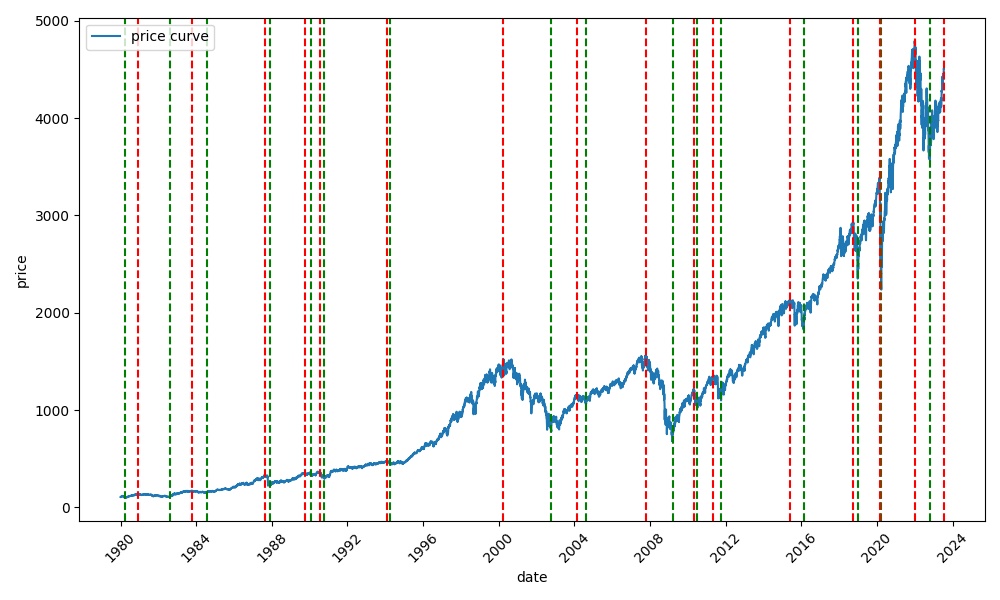
\includegraphics[width=0.8\linewidth]{chapters/chapter1/figures/curve_GSPC_126D}
	\caption{S\&P 500 Index: curve and trend identification based on 126-day horizon.}
	\label{fig:curvegspc126d}
\end{figure}

\begin{figure}[h]
	\centering
	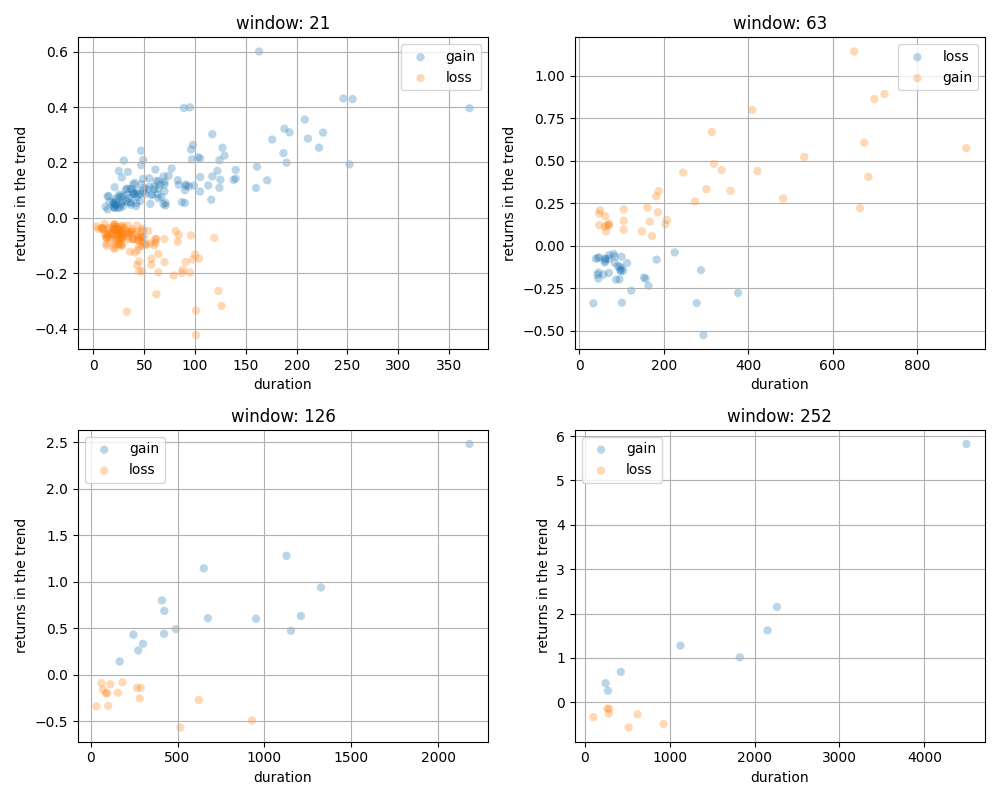
\includegraphics[width=1\linewidth]{chapters/chapter1/figures/scatter_GSPC}
	\caption{Scatter plots of the returns and durations of the trend for S\&P 500 index, with different horizons.}
	\label{fig:scattergspc}
\end{figure}

\subsubsection{Dow Jones Industrial 30}


\begin{figure}[h]
	\centering
	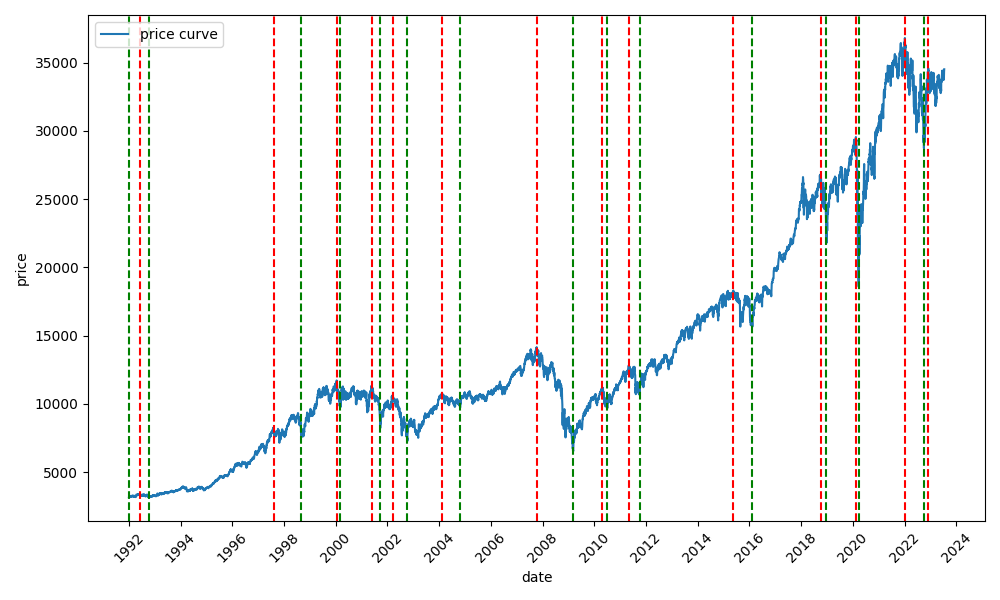
\includegraphics[width=0.8\linewidth]{chapters/chapter1/figures/curve_DJI_126D}
	\caption{DJI Index: curve and trend identification based on 126-day horizon.}
	\label{fig:curvedji126d}
\end{figure}

\begin{figure}[h]
	\centering
	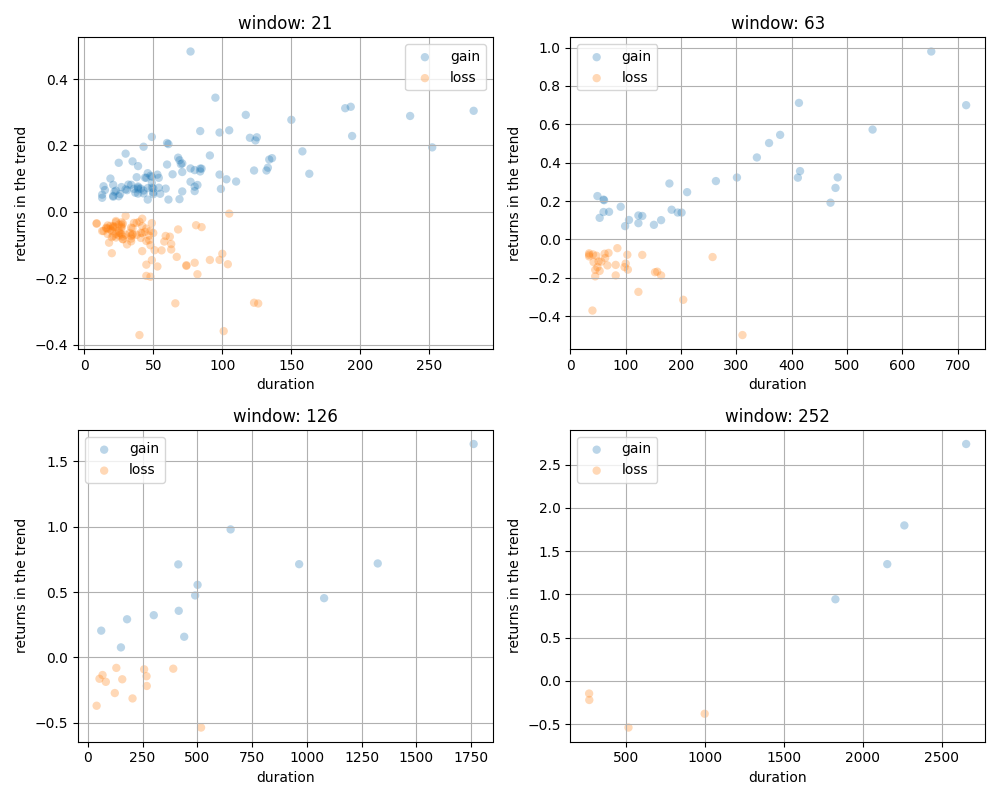
\includegraphics[width=1\linewidth]{chapters/chapter1/figures/scatter_DJI}
	\caption{Scatter plots of the returns and durations of the trend for DJI index, with different horizons.}
	\label{fig:scatterdji}
\end{figure}

